\documentclass[12pt]{article}
\setlength{\oddsidemargin}{0in}
\setlength{\evensidemargin}{0in}
\setlength{\textwidth}{6.5in}
\setlength{\parindent}{0in}
\setlength{\parskip}{\baselineskip}

\usepackage{amsmath,amsfonts,amssymb}
\usepackage{booktabs,multirow}
\usepackage{tikz}

\title{CMSC 471 - HW3}

\begin{document}

CMSC 471 Spring 2018\hfill Homework \#3: Chapter 3\\
Robert Rose

\hrulefill

\begin{enumerate}
\item \textbf{3.15} Consider a state space where the start state is number 1 and each state is $k$ has two successors: the numbers $2k$ and $2k + 1$
  \begin{enumerate}
  \item Draw the portion of the state space for states 1 to 15.
  \begin{center}
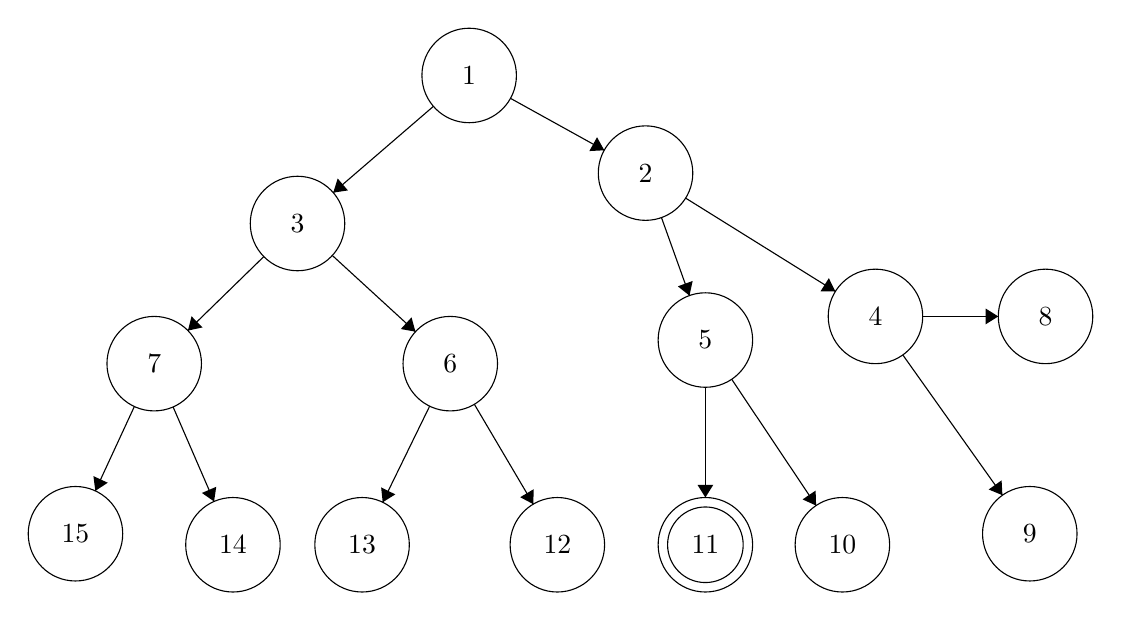
\begin{tikzpicture}[scale=0.2]
\tikzstyle{every node}+=[inner sep=0pt]
\draw [black] (29.7,-6.7) circle (3);
\draw (29.7,-6.7) node {$1$};
\draw [black] (40.9,-12.9) circle (3);
\draw (40.9,-12.9) node {$2$};
\draw [black] (18.8,-16.1) circle (3);
\draw (18.8,-16.1) node {$3$};
\draw [black] (55.5,-22) circle (3);
\draw (55.5,-22) node {$4$};
\draw [black] (44.7,-23.5) circle (3);
\draw (44.7,-23.5) node {$5$};
\draw [black] (28.5,-25) circle (3);
\draw (28.5,-25) node {$6$};
\draw [black] (9.7,-25) circle (3);
\draw (9.7,-25) node {$7$};
\draw [black] (66.3,-22) circle (3);
\draw (66.3,-22) node {$8$};
\draw [black] (65.3,-35.8) circle (3);
\draw (65.3,-35.8) node {$9$};
\draw [black] (53.4,-36.5) circle (3);
\draw (53.4,-36.5) node {$10$};
\draw [black] (44.7,-36.5) circle (3);
\draw (44.7,-36.5) node {$11$};
\draw [black] (44.7,-36.5) circle (2.4);
\draw [black] (35.3,-36.5) circle (3);
\draw (35.3,-36.5) node {$12$};
\draw [black] (22.9,-36.5) circle (3);
\draw (22.9,-36.5) node {$13$};
\draw [black] (14.7,-36.5) circle (3);
\draw (14.7,-36.5) node {$14$};
\draw [black] (4.7,-35.8) circle (3);
\draw (4.7,-35.8) node {$15$};
\draw [black] (32.32,-8.15) -- (38.28,-11.45);
\fill [black] (38.28,-11.45) -- (37.82,-10.62) -- (37.33,-11.5);
\draw [black] (41.91,-15.72) -- (43.69,-20.68);
\fill [black] (43.69,-20.68) -- (43.89,-19.75) -- (42.95,-20.09);
\draw [black] (43.45,-14.49) -- (52.95,-20.41);
\fill [black] (52.95,-20.41) -- (52.54,-19.57) -- (52.01,-20.41);
\draw [black] (16.66,-18.2) -- (11.84,-22.9);
\fill [black] (11.84,-22.9) -- (12.77,-22.7) -- (12.07,-21.99);
\draw [black] (58.5,-22) -- (63.3,-22);
\fill [black] (63.3,-22) -- (62.5,-21.5) -- (62.5,-22.5);
\draw [black] (57.24,-24.45) -- (63.56,-33.35);
\fill [black] (63.56,-33.35) -- (63.51,-32.41) -- (62.69,-32.99);
\draw [black] (46.37,-25.99) -- (51.73,-34.01);
\fill [black] (51.73,-34.01) -- (51.7,-33.06) -- (50.87,-33.62);
\draw [black] (44.7,-26.5) -- (44.7,-33.5);
\fill [black] (44.7,-33.5) -- (45.2,-32.7) -- (44.2,-32.7);
\draw [black] (27.43,-8.66) -- (21.07,-14.14);
\fill [black] (21.07,-14.14) -- (22,-14) -- (21.35,-13.24);
\draw [black] (30.03,-27.58) -- (33.77,-33.92);
\fill [black] (33.77,-33.92) -- (33.8,-32.97) -- (32.94,-33.48);
\draw [black] (10.9,-27.75) -- (13.5,-33.75);
\fill [black] (13.5,-33.75) -- (13.64,-32.82) -- (12.73,-33.21);
\draw [black] (21.01,-18.13) -- (26.29,-22.97);
\fill [black] (26.29,-22.97) -- (26.04,-22.06) -- (25.36,-22.8);
\draw [black] (27.19,-27.7) -- (24.21,-33.8);
\fill [black] (24.21,-33.8) -- (25.01,-33.3) -- (24.11,-32.86);
\draw [black] (8.44,-27.72) -- (5.96,-33.08);
\fill [black] (5.96,-33.08) -- (6.75,-32.56) -- (5.84,-32.14);
\end{tikzpicture}
\end{center}
  \item Suppose the goal state is 11. List the order in which nodes will be visited for breadth-first search, depth-limited search with limit 3, and iterative deepening search.
  \begin{enumerate}
  \item \textbf{Breadth-First Search}: 1, 2, 3, 4, 5, 10, \textbf{11}
  \item \textbf{Depth-Limited Search}: 1, 2, 4, 8, 9, 5, 10, \textbf{11}
  \item \textbf{Iterative Deepening Search}: \{1\}, \{1, 2, 3\}, \{1, 2, 3, 4, 5, 6, 7\}, \{1, 2, 3, 4, 5, 6, 7, 8, 9, 10, \textbf{11}\}
  \end{enumerate}
  \item How well would bidirectional search work on this problem? What is the branching factor in each direction of the bidirectional search?\\
  \vspace{-2.5em}
  \paragraph{Well.} It would work rather well as there is a sole starting and final state and there is only one path between them. Branching factor would be 2.
  \item Does the answer to (c) suggest a reformulation of the problem that would allow you to solve the problem of getting from state 1 to a given goal state with almost no search?\\
  \vspace{-2.5em}
  \paragraph{Yes} This is effectively a binary search tree so we could just keep going to whatever branch has a higher state less than 11.
  \item Call the action going from $k$ to $2k$ Left, and the action from going to $2k + 1$ Right. Can you find an algorithm that outputs the solution to this problem without any search at all?\\
  \vspace{-2.5em}
  \paragraph{Yes} The path between 1 and 11 will be Left, Right, Right.
  \end{enumerate}

\item \textbf{3.26} Consider the unbounded version of the regular 2D grid shown in Figure 3.9. The start state is at the origin, (0,0), and the goal state is at ($x$, $y$).
  \begin{enumerate}
  \item What is the branching factor $b$ in this state space?
  \item How many distinct states are there at depth $k$ (for $k > 0$)?
  \item What is the maximum number of nodes expanded by breadth-first tree search?
  \item What is the maximum number of nodes expanded by breadth-first graph search?
  \item Is $h = \left|u - x\right| + \left|v - y\right|$ an admissible heuristic for a state at ($u, v$)? Explain.
  \item How many nodes are expanded by A* graph search using $h$?
  \item Does $h$ remain admissible if some links are removed?
  \item Does $h$ remain admissible if some links are added between nonadjacent states?
  \end{enumerate}

\end{enumerate}
\end{document}